
  \section{Zielsetzung}
  Der Versuch dient zum einen zur Untersuchung eines Reflexklystrons.
  Zum anderen soll die Frequenz, die Wellenlänge und die Dämpfung bestimmt werden.
  Ein weiteres Ziel ist die Welligkeitsmessung.

  \section{Theorie}

  Mikrowellen decken den Frequenzbereich von ca. 300\,MHz bis 300\,GHz ab.
  Diese elektromagnetischen Wellen können mit einem Hohlleiter weitergeleitet werden.
  Jeder Wellentyp (Mode) hat eine Grenzfrequenz unter der kein Energietransport durh den Hohlleiter mehr stattfindet.
  Sie ist abhängig von den Maßen des Hohlleiters.
  Es wird zwischen zwei Moden unterschieden:\\
  Transversal elektrische und magnetische Moden.
  Diese Moden haben ein elektrisches bzw. magnetisches Feld, dass senkrecht zur Fortpflanzungsrichtung ist.

  Ein Klystron ist eine Mikrowellenröhre, in der durch Geschwindigkeitsmodulation Mikrowellenenergie gewonnen wird.
  An dem Reflektor liegt ein gegen die Kathode negatives Potential an, weshalb die emittierten Elektronen von ihm reflektiert werden.
  Sie laufen durch das Resonatorgitter und mit Hilfe des Klystrons wird das System zum schwingen gebracht.
  Die Elektronen verlassen den Resonator entweder beschleunigt oder abgebremst, sodass sie einen Geschwindigkeitsunterschied haben.
  Daraus folgt, dass sich die rückkehrenden Elektronen zu einem Bündel vereinigen.
  Dieser Bündel tritt in Wechselwirkung mit dem Feld und gibt so Energie an den Resonator ab.
  Bei n+ $\sfrac{3}{4}$ Perioden Gangunterschied tritt dabei die stärkste Verstärkung auf.

  Der Zusammenhang zwischen Frequenz und Wellenlänge kann im freien Raum beschrieben werden durch
  \begin{equation*}
    c = f \cdot\lambda_0.
  \end{equation*}
  Im luftgefüllten Hohlleiter gilt
  \begin{equation}
    \lambda_g = \frac{\lambda_0}{\sqrt{1-\left(\frac{\lambda_0}{\lambda_e}\right)^2}}.
  \end{equation}
  $\lambda_e$ beschreibt dabei die Grenzwellenlänge im Hohlleiter.
  Sie entspricht zwei mal der Breitseite des Hohlleiters,
  für die Frequenz ergibt sich somit
  \begin{equation}
    f = c\cdot \sqrt{\left(\frac{1}{\lambda_g}\right)^2+\left(\frac{1}{2a}\right)^2}.
    \label{eqn:1}
  \end{equation}

  An jedem Punkt der Hohlleitung kann die Welle als eine vom Generator emittierten und einer reflektierten Welle aufgefasst werden.
  Die reflektierte Welle entsteht durch Unebenheiten im Hohleiter oder an einer Lastimpedanz.
  Haben beide Wellen die gleiche Phasenlage, wird die Feldstärke maximal.
  Das Verhältnis zwischen den elektrischen Feldstärken der emittierten und reflektierten Welle wird als Spannungs-Reflexionskoeffizient $\rho$ beschrieben.
  Das "Spannungs-Stehwellen-Verhältnis"(SWR) wird durch den Quotienten aus maximaler und minimaler Feldstärke berechnet.\\
  Es gibt mehrere Messverfahren zur Bestimmung von Welligkeiten.
  Zum einen die direkte Messung, die bei hohem SWR ungenau wird, und zum anderen die "3-dB-Methode".
  Das SWR wird berechnet mit
  \begin{align}
    S &= \sqrt{1 + \frac{1}{\sin^2\left(\frac{\pi (d_1-d_2)}{\lambda_g}\right)}}\\
      &\approx \frac{\lambda_g}{\pi (d_1-d_2)}.
    \label{eqn:2}
  \end{align}
  Der zweite Teil ist eine Nährung, die angewandt werden kann, wenn S größer als 10 ist.
  Bei der "3-dB-Methode" kommt es zu Abweichungen des Detektors vom quadratischen Verhalten der Diode.
  Dieses wird mit der "Abschwächer-Methode" überwunden.
  Das Ausgangssignal im Maximum wird dem im Minimum gleichgesetzt.



  \section{Durchführung}
    \subsection{Untersuchung eines Reflexklystrons}
    Zunächst wird die Apparatur wie in Abbildung \ref{fig:Aufbauklystron} zu sehen aufgebaut.
    \begin{figure}
      \centering
      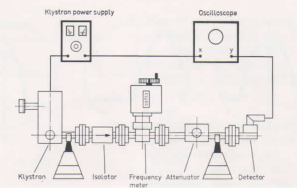
\includegraphics[scale = 0.8]{pictures/aufbauKlystron.png}
      \caption{Aufbau für die Klystron-Untersuchungen mit dem Oszillographen\cite{anleitung}}
      \label{fig:Aufbauklystron}
    \end{figure}
    Das Dämpfungsglied wird auf 30\,dB gestellt.
    Die Amplitude der Sinusspannung wird so eingestellt, dass sich eine horizontale Linie parallel zur Mittellinie ergibt.
    Die Reflektorspannung wird auf etwa 200\,V eingestellt und so lange variiert, bis die Modenkurven im Mittelpunkt liegen.
    Der Frequenzmesser wird so abgestimmt, dass eine Sattelung an der Spitze der Kurve erscheint, wie in Abbildung \ref{fig:Mode} zu sehen.
    Die Frequenz und die Spannung wird aufgenommen und die Kurve nach rechts bzw links verschoben,
    wie in Abbildung \ref{fig:Mode} zu sehen, und diejenigen Spannungen werden wieder aufgenommen.
    Außerdem wird die Amplitude bestimmt.
    \begin{figure}
      \centering
      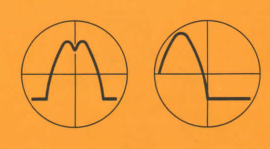
\includegraphics[scale=0.8]{pictures/Mode.png}
      \caption{Mode mit Einsattelung und Verschiebung\cite{anleitung}}
      \label{fig:Mode}
    \end{figure}
    Nun wird der Frequenzmesser verstimmt und die Resonatorspannung neu abgestimmt,
    sodass das Maximum des Modus im Mittelpunkt liegt.
    Auch hier werden Spannungen, die Amplitude und die Frequenz für die drei Einstellungen aus Abbildung \ref{fig:Mode2}
    bestimmt.
    \begin{figure}
      \centering
      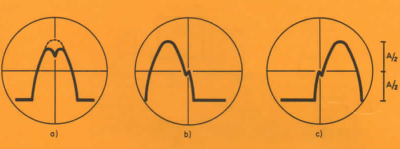
\includegraphics[scale = 0.8]{pictures/Mode2.png}
      \caption{Abgleich der Reflektorspannug nach den Abbildungen a) - c)\cite{anleitung}}
      \label{fig:Mode2}
    \end{figure}

    \subsection{Messung von Frequenz, Wellenlänge und Dämpfung}
    Die Apparatur wird nach Abbildung \ref{fig:aufbauv2} geändert, sodass der Abschluss angebaut ist.
    \begin{figure}
      \centering
      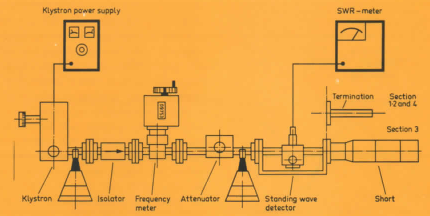
\includegraphics[scale=0.8]{pictures/AufbauV2.png}
      \caption{Aufbau zum zweiten Versuchsteil\cite{anleitung}}
      \label{fig:aufbauv2}
    \end{figure}
    Das Dämpfungsglied wird auf 20\,dB gestellt und die Reflektorspannung auf ca. 200\,V.
    Am SWR-Meter werden 40\,dB und eine Bandbreite von 100\,Hz eingestellt.
    Mit dem 1\,kHz Regler wird ein maximaler Ausschlag erzeugt.
    Danach wird der Frequenzmesser so verändert, dass es zu einem minimalen Ausschlag kommt.\\
    Nun wird der Abschluss durch den verstellbaren Kurzschluss ersetzt und der Frequenzmessser verstimmt.
    Mit der Sonde werden nun die Punkte des minimalen Ausschlags gesucht.\\
    Der Kurzschluss wird wieder durch den Abschluss ersetzt und der Frequenzmesser auf 9000\,MHz gestellt.
    Die Verstärkung des SWR-Meters wird auf den maximalen Ausschlag gedreht.
    Das Dämpfungsglied wird zunächst so gestellt, dass keine Dämpfung vorliegt.
    Dann wird die Dämpfung immer weiter verstärkt um das Verhältnis zwischen mm und dB zu erhalten.
    Dies wird bis 10\,dB durchgeführt.

    \subsection{Stehwellen-Messungen}
    Für die Messung der Welligkeiten wird der Versuchsaufbau nach Abbildung \ref{fig:aufbauV3} verändert.
    \begin{figure}
      \centering
      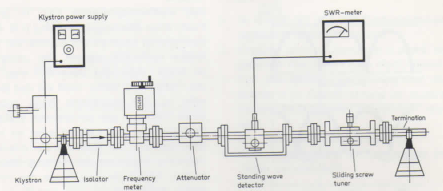
\includegraphics[scale=0.8]{pictures/aubauV3.png}
      \caption{Aufbau zur Stehwellen-Messung}
      \label{fig:aufbauV3}
    \end{figure}
    Der Abschwächer wird fest auf 20\,dB eingestellt und am SWR-Meter werden 40\,dB und eine Bandbreite von 20\,Hz eingestellt.
    Das System wird bei 9\,GHz mit Hilfe des Klystrons zum Schwingen gebracht.
    Nun werden die kleinen und mittleren Welligkeiten gemessen.
    Dafür wird zunächst die Sondentiefe des Gleitschraubentransformators auf 3, 5, 7 und 9\,mm gestellt und ein Maximum sowie ein Minimum gesucht.

    Mit der "3 dB-Methode" werden nun die großen Welligkeiten gemessen.
    Die Sonde wird auf 9\,mm gestellt und es wird wieder ein Minimum gesucht.
    Mit dem Verstärker wird die Anzeige dann auf 3\,dB geregelt.
    Die Sonde der Messleitung wird dann einmal nach recht und einmal nach links verschoben bis sich ein Vollausschlag ergibt.
    Jetzt wird wieder der Kurzschluss eingebaut und der Abstand zwischen den Minima gemessen.

    Die großen Welligkeiten werden nun mit der "Abschwächer-Methode" bestimmt.
    Die ersten Schritte von der vorherigen Methode werden wiederholt.
    Zusätzlich wird nun allerdings das Dämpfungsglied auf 20\,dB gesetzt bevor auf 3\,dB justiert wird.
    Durch Veränderung des Dämpfungsglied bei Verschieben der Messleitung wird das relative Maximum bestimmt.
